% Editable primary source. Build: latexmk -pdf phast_autumn_school_2026.tex
% Course material created by Allamaprabhu Ani, CEMS-Lab, UKACM Autumn School 2026.
% Generate original figures first: python build_beamer_figures.py
\documentclass[aspectratio=169,12pt,usepdftitle=false]{beamer}
\usepackage[T1]{fontenc}
\usepackage{lmodern,amsmath,amssymb,booktabs,graphicx,tikz,listings,array}
\usetikzlibrary{arrows.meta,positioning,calc,shapes.geometric}
\usefonttheme[onlymath]{serif}
\definecolor{navy}{HTML}{20364D}
\definecolor{teal}{HTML}{087F82}
\definecolor{muted}{HTML}{67737D}
\definecolor{rust}{HTML}{BD5435}
\definecolor{forward}{HTML}{245A81}
\definecolor{reverse}{HTML}{B85C20}
\tikzset{process/.style={draw=forward,fill=forward!4,minimum height=9mm,
  text width=2.1cm,align=center,font=\normalsize,inner sep=3mm},
  state/.style={circle,draw=forward,fill=white,minimum size=9mm,inner sep=2mm},
  flow/.style={-{Latex[length=2.5mm]},draw=forward,line width=1pt},
  backflow/.style={-{Latex[length=2.5mm]},draw=reverse,line width=1pt},
  decision/.style={diamond,aspect=2.1,draw=navy,fill=white,align=center,
    inner sep=1mm,font=\small}}
\setbeamercolor{normal text}{fg=black,bg=white}
\setbeamercolor{frametitle}{fg=black,bg=white}
\setbeamercolor{structure}{fg=teal}
\setbeamerfont{frametitle}{size=\Large,series=\mdseries}
\setbeamersize{text margin left=9mm,text margin right=9mm}
\setbeamertemplate{navigation symbols}{}
\setbeamertemplate{itemize item}{\color{teal}\small$\bullet$}
\setbeamertemplate{footline}{\hfill\color{muted}\tiny\insertframenumber\hspace{9mm}\vspace{3mm}}
\setbeamertemplate{frametitle}{\vspace{5mm}\insertframetitle\par\vspace{2mm}}
\setbeameroption{hide notes}
\hypersetup{colorlinks=true,urlcolor=teal,pdftitle={From cracks to computation},pdfauthor={Allamaprabhu Ani},pdfsubject={CEMS-Lab, UKACM Autumn School 2026; presented by Sathiskumar A. Ponnusami, Queen Mary University of London}}
\title{From cracks to computation}
\author{Sathiskumar A. Ponnusami}
\newcommand{\source}[1]{\vfill{\color{muted}\fontsize{6.4}{7.4}\selectfont #1\par}}
\newcommand{\question}[1]{\note{Discussion prompt: #1}}
\newcommand{\tagline}[1]{{\color{muted}\scriptsize #1}\par\vspace{2mm}}
\newcommand{\fig}[2][.95]{\includegraphics[width=#1\linewidth]{latex_figures/#2.pdf}}
\newcommand{\timing}[2]{\note{\textbf{#1.} #2}}
\newcommand{\fm}{Francfort \& Marigo (1998), \href{https://doi.org/10.1016/S0022-5096(98)00034-9}{JMPS 46, 1319--1342}.}
\newcommand{\bfm}{Bourdin, Francfort \& Marigo (2000), \href{https://doi.org/10.1016/S0022-5096(99)00028-9}{JMPS 48, 797--826}.}
\newcommand{\miehe}{Miehe, Welschinger \& Hofacker (2010), \href{https://doi.org/10.1002/nme.2861}{IJNME 83, 1273--1311}.}
\newcommand{\pham}{Pham et al. (2011), \href{https://doi.org/10.1177/1056789510386852}{IJDM 20, 618--652}.}
\newcommand{\phast}{\href{https://github.com/CEMS-Lab/PhAST}{PhAST source and documentation}.}
\newcommand{\ad}{\href{https://docs.pytorch.org/docs/autograd}{PyTorch autograd documentation}.}
\newcommand{\daggerref}{Ross, Gordon \& Bagnell (2011), \href{https://proceedings.mlr.press/v15/ross11a.html}{AISTATS: dataset aggregation}.}
\newcolumntype{L}[1]{>{\raggedright\arraybackslash}p{#1}}
\newcommand{\flowfour}[4]{\begin{center}\begin{tikzpicture}[>=Latex, every node/.style={align=center,text width=2.7cm,font=\large}]
\node (a) at (0,0) {#1};\node (b) at (3.35,0) {#2};\node (c) at (6.70,0) {#3};\node (d) at (10.05,0) {#4};
\draw[->,teal,thick] (a)--(b);\draw[->,teal,thick] (b)--(c);\draw[->,teal,thick] (c)--(d);\end{tikzpicture}\end{center}}
\newcommand{\session}[4]{\begin{frame}{#1}\tagline{#2}\vspace{6mm}{\LARGE #3\par}\vspace{7mm}{\color{muted}120 minutes, including a 10-minute break\par}\timing{#2}{#4}\end{frame}}
\lstset{basicstyle=\ttfamily\small,keywordstyle=\color{teal},commentstyle=\color{muted},showstringspaces=false,columns=fullflexible,keepspaces=true,breaklines=true}
\ifdefined\Preview\includeonlyframes{cover,energy,degradation}\fi
\begin{document}

\begin{frame}[label=cover,plain]
\begin{columns}[c]
\begin{column}{.63\textwidth}
\tagline{PhAST / UKACM Autumn School 2026}
{\fontsize{29}{33}\selectfont\bfseries From cracks\\to computation\par}
\vspace{6mm}
{\large Phase-field fracture, differentiable\\FEM and learning with PhAST\par}
\vspace{8mm}
{\color{muted}Sathiskumar A. Ponnusami\\Queen Mary University of London\\CEMS-Lab}
\end{column}
\begin{column}{.35\textwidth}
\fig[1]{title_specimen}
{\centering\color{muted}\scriptsize Phase-field representation (schematic)\par}
\end{column}
\end{columns}
\timing{Opening}{Introduce the 2+2+2-hour design. Each section includes a ten-minute break. The event allocation is separate and must be agreed with the organiser. The title illustration shows an analytic distance-based representation of a crack.}
\end{frame}

\begin{frame}{Six hours: understand, compute, then learn}
\begin{center}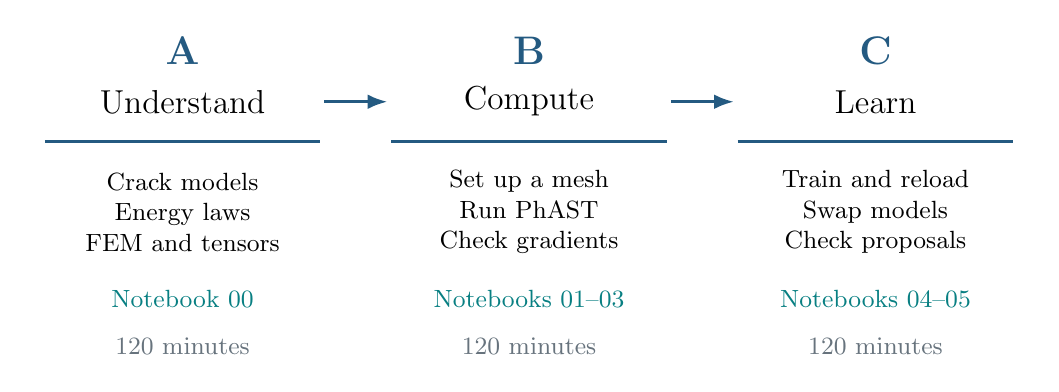
\begin{tikzpicture}[>=Latex]
\foreach \x/\letter/\label in {0/A/Understand,4.4/B/Compute,8.8/C/Learn}{
  \node[font=\Large\bfseries,text=forward] at (\x,1.6) {\letter};
  \node[font=\large] at (\x,.95) {\label};
  \draw[forward,line width=1pt] (\x-1.75,.45)--(\x+1.75,.45);
  \node[muted,font=\small] at (\x,-2.15) {120 minutes};}
\node[align=center,text width=3.7cm,font=\small] at (0,-.45) {Crack models\\Energy laws\\FEM and tensors};
\node[align=center,text width=3.7cm,font=\small] at (4.4,-.45) {Set up a mesh\\Run PhAST\\Check gradients};
\node[align=center,text width=3.7cm,font=\small] at (8.8,-.45) {Train and reload\\Swap models\\Check proposals};
\node[teal,font=\small] at (0,-1.55) {Notebook 00};
\node[teal,font=\small] at (4.4,-1.55) {Notebooks 01--03};
\node[teal,font=\small] at (8.8,-1.55) {Notebooks 04--05};
\draw[flow] (1.8,.95)--(2.6,.95);\draw[flow] (6.2,.95)--(7,.95);
\end{tikzpicture}\end{center}
\question{Take away one executed notebook and one comparison sheet.}
\source{Six-hour session design: 330 minutes of teaching and activity, with 30 minutes of breaks.}
\timing{Orientation}{Introduce the companion book and notebook routes. Notebook 01 is a real PhAST damage-evolution solve; notebooks 02--05 teach local differentiation, an elastic-bar inverse toy and a Helmholtz-like field model/adapter. The distinctions remain visible throughout.}
\end{frame}

\session{Understand the crack}{Session A / 00--10}{Read a damage field.\\Explain the energy.\\Trace one numerical increment.}{Ten-minute opening prediction activity. Ask where a centreline precrack in tension will localise damage. Damage describes a diffuse material state. Displacement jumps and crack opening describe kinematics. A schematic can support a hypothesis; an actual field and its loading history are needed to test it.}

\begin{frame}{Three descriptions of an evolving crack}
\hspace*{.03\textwidth}\fig[.94]{representations}
\begin{columns}[t]
\begin{column}{.31\textwidth}\small XFEM enriches the approximation around a sharp discontinuity.\end{column}
\begin{column}{.31\textwidth}\small A cohesive law relates interface traction to separation.\end{column}
\begin{column}{.31\textwidth}\small Phase field adds damage $d$ and length scale $\ell$.\end{column}
\end{columns}
\question{An adhesive interface? An unknown branching path?}
\source{Original schematics; these approaches can be combined. \miehe}
\timing{A 10--22 / 12 minutes}{Compare the same conceptual specimen. XFEM enriches the approximation, while a cohesive law relates traction to separation. A phase-field-CZM exists. Discuss interface knowledge, path complexity, calibration and computational cost without claiming universal superiority.}
\end{frame}

\begin{frame}{Fracture models and solution algorithms}
\begin{tabular}{@{}L{.32\textwidth}L{.62\textwidth}@{}}
\toprule
Question & Examples\\\midrule
What does the crack mean? & Sharp surface, cohesive relation, diffuse field\\[4mm]
How is it discretised? & FE spaces, enrichment, mesh, quadrature\\[4mm]
How is it solved? & Staggered/monolithic; Newton/quasi-Newton\\\bottomrule
\end{tabular}
\question{Can quasi-Newton solve a phase-field system?}
\source{Quasi-Newton methods solve nonlinear equations within a chosen crack model.}
\timing{A 22--25 / 3 minutes}{Use the question for retrieval. Classify each term before describing advantages. Distinguish an FE enrichment from the physical constitutive relation and the nonlinear algorithm.}
\end{frame}

\begin{frame}[label=energy]{Fracture balances storage and crack cost}
\tagline{A representative small-strain brittle model}
\vspace{-2mm}
\begin{align*}
\mathcal E_\ell(u,d)
&=\underbrace{\int_\Omega\!\left[g(d)\psi^+(\varepsilon(u))+\psi^-(\varepsilon(u))\right]\,\mathrm dx}_{\text{elastic energy: damage reduces tensile storage}}\\[5mm]
&\quad+\underbrace{\frac{G_c}{c_0}\int_\Omega\!\left[\frac{w(d)}{\ell}+\ell\lvert\nabla d\rvert^2\right]\,\mathrm dx}_{\text{crack cost: local damage + spatial regularisation}}
\; -\;\underbrace{W_{\rm ext}}_{\text{loading}}.
\end{align*}
\question{Which term favours damage? Which term resists it?}
\source{\fm\quad\bfm\quad Split shown is representative; dynamic mechanics also requires inertia.}
\timing{A 25--37 / 12 minutes}{Build the two lines term by term. Define displacement u, small strain, damage d, toughness Gc and length ell. The normalisation is c0=4 integral from 0 to 1 of sqrt(w(s)) ds. This representative model uses a tension/compression energy split. Ask learners to identify storage reduction and crack cost.}
\end{frame}

\begin{frame}{AT1 and AT2 choose the crack-density term}
\[
c_0=4\int_0^1\sqrt{w(s)}\,\mathrm ds
\]
\vspace{-1mm}
\begin{columns}[t]
\begin{column}{.46\textwidth}
{\color{teal}AT1}\[w(d)=d,\qquad c_0=\frac83\]
\small Finite elastic stage in the standard idealisation.
\end{column}
\begin{column}{.46\textwidth}
{\color{teal}AT2}\[w(d)=d^2,\qquad c_0=2\]
\small Gradual early damage in the standard idealisation.
\end{column}
\end{columns}
\vspace{-1mm}
\[\underbrace{d=0}_{\text{intact}}\qquad\underbrace{d=1}_{\text{broken}}\qquad d_{n+1}\ge d_n\]
\source{Degradation $g(d)$ is a separate choice. \pham}
\timing{A 37--45 / 8 minutes}{Compute c0 for w=d and w=d squared. Note that onset also depends on degradation, split, loading, flaw, length and calibration. The statement about an elastic stage applies to these standard idealisations. Maintain the d=0 intact convention consistently.}
\end{frame}

\begin{frame}[label=degradation]{How quickly should stiffness be lost?}
\begin{columns}[c]
\begin{column}{.26\textwidth}
\small Quadratic baseline
\[\begin{aligned}g(d)&=(1-\eta)(1-d)^2\\&\quad+\eta\end{aligned}\]
\[g(0)=1\]
\[g(1)=\eta\]
\end{column}
\begin{column}{.72\textwidth}\fig[1]{degradation}\end{column}
\end{columns}
\source{Analytic degradation curves with $\eta=10^{-6}$; notebooks 01 and 02 use $\eta=10^{-7}$.}
\timing{A 45--53 / 8 minutes}{Predict before explaining. Quadratic law exactly matches the selected PhAST baseline. Cubic illustration: (1-eta)(1-3d squared+2d cubed)+eta. Rational illustration: (1-eta)(1-d) squared/[(1-d) squared+a d(1+d)]+eta, a=2. For a>0 its denominator is positive on [0,1]. Use the cubic and rational curves as illustrative degradation choices.}
\end{frame}

\begin{frame}{A derivative measures the local energy response}
\begin{columns}[c]
\begin{column}{.28\textwidth}
\small
\[\begin{aligned}g'(d)&=-2(1-\eta)\\&\quad\cdot(1-d)\end{aligned}\]
\[g''(d)=2(1-\eta)\]
\question{Why is $g'$ negative?}
\end{column}
\begin{column}{.70\textwidth}\fig[1]{degradation_derivative}\end{column}
\end{columns}
\source{Analytic sensitivity of the local degradation law.}
\timing{A 53--60 / 7 minutes, then break 60--70}{Predict g prime at d=0.25. The illustrative plot uses eta=1e-6, giving -1.4999985. Notebook 02 uses eta=1e-7, giving -1.49999985. Explain local AD and later revisit the full computational path. Take the ten-minute comfort break.}
\end{frame}

\begin{frame}{A diffuse crack has a spatial profile}
\begin{columns}[c]
\begin{column}{.28\textwidth}
\small AT2\[d=e^{-|x|/\ell}\]
AT1\[d=\left[1-\frac{|x|}{2\ell}\right]_+^2\]
\question{Tail or compact support?}
\end{column}
\begin{column}{.70\textwidth}\fig[1]{damage_profiles}\end{column}
\end{columns}
\source{Isolated one-dimensional crack-density minimisers with $d(0)=1$. \pham}
\timing{A 70--78 / 8 minutes}{Read the horizontal axis as x/ell. Explain exponential tail versus compact support and how ell scales both. These profiles minimise the isolated crack-density functional.}
\end{frame}

\begin{frame}{The mesh must resolve the chosen length}
\fig[1]{mesh_resolution}
\[\ell\;:\;\text{model scale}\qquad\qquad h\;:\;\text{discretisation scale}\]
\question{Refine $h$ at fixed $\ell$. What should you compare?}
\source{The same analytic damage band on two schematic meshes; resolution is measured relative to $\ell$.}
\timing{A 78--85 / 7 minutes}{Ask whether one element across a band can describe it. Hold ell and physical parameters fixed while refining h. Compare full damage fields, load response and energies. Changing ell can alter nucleation/strength and requires separate calibration. Assess mesh convergence through systematic refinement.}
\end{frame}

\begin{frame}{Crack initiation, propagation and branching}
\fig[1]{evolution_schematic}
\begin{columns}[t]
\begin{column}{.31\textwidth}\small Where does damage first grow?\end{column}
\begin{column}{.31\textwidth}\small Where does an existing crack advance?\end{column}
\begin{column}{.31\textwidth}\small When does one path become two?\end{column}
\end{columns}
\source{Schematic stages of crack initiation, growth and branching.}
\timing{A 85--90 / 5 minutes}{The three sketches illustrate separate conceptual crack states. Discuss flaw, strength, loading and regularisation. Dynamic branching requires a physical time history and a converged path-instability calculation. Notebook 01 demonstrates quasistatic damage evolution.}
\end{frame}

\begin{frame}{A staggered step alternates coupled problems}
\tagline{Fix the load increment $n$; iterate the coupled fields with index $k$}
\begin{center}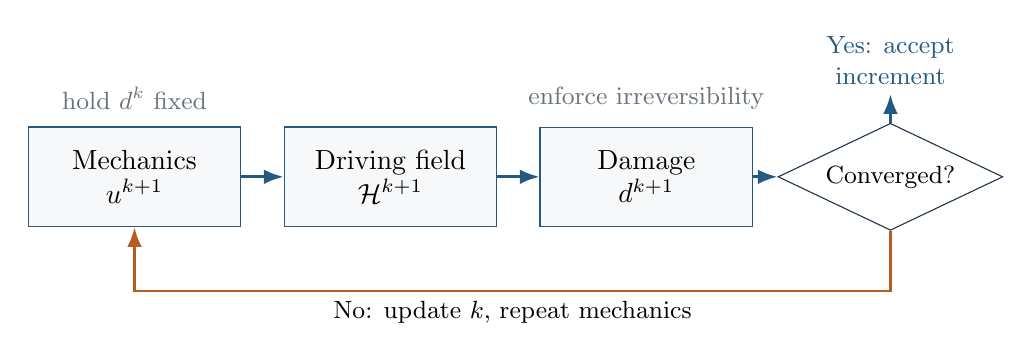
\begin{tikzpicture}[>=Latex]
\node[process] (u) at (0,0) {Mechanics\\$u^{k+1}$};
\node[process] (h) at (3.25,0) {Driving field\\$\mathcal H^{k+1}$};
\node[process] (d) at (6.5,0) {Damage\\$d^{k+1}$};
\node[decision] (q) at (9.6,0) {Converged?};
\draw[flow] (u)--(h);\draw[flow] (h)--(d);\draw[flow] (d)--(q);
\node[muted,font=\small] at (0,1) {hold $d^k$ fixed};
\node[muted,font=\small] at (6.5,1) {enforce irreversibility};
\draw[backflow] (q.south)--(9.6,-1.45)--node[below,font=\small]{No: update $k$, repeat mechanics}(0,-1.45)--(u.south);
\draw[flow] (q.north)--(9.6,1.05);
\node[anchor=south,align=center,font=\small,text=forward] at (9.6,1.05) {Yes: accept\\increment};
\end{tikzpicture}\end{center}
\question{Which field is held fixed in each subproblem?}
\source{History-field notation is representative; irreversibility and the convergence criterion depend on the selected formulation. \miehe}
\timing{A 90--100 / 10 minutes}{Trace an outer load increment and inner staggered iterations. Mechanics uses current damage; the driving/history field depends on tensile energy; damage uses updated driving. Keep prescribed damage and irreversibility. Advance only under the chosen convergence checks. The gradient term has a diffusion-like structure. Damage evolution additionally reflects fracture energy and irreversibility.}
\end{frame}

\begin{frame}{Time integration and nonlinear iteration are different}
\[\underbrace{\mathbf M\ddot{\mathbf u}}_{\text{inertia}}+\mathbf r_{\rm int}(\mathbf u,d)=\mathbf f_{\rm ext}\]
\small
\begin{tabular}{@{}L{.28\textwidth}L{.66\textwidth}@{}}
Static/quasi-static & Equilibrium along a prescribed load path.\\[3mm]
Explicit mechanics & Central difference/Verlet; stability limits the time step.\\[3mm]
Implicit mechanics & Newmark/generalised-$\alpha$; solve an implicit update.\\[3mm]
Newton/quasi-Newton & Iterations for a nonlinear algebraic system.\\
\end{tabular}
\source{An explicit mechanics update can still use an implicit damage solve. Notebook 01 follows a quasi-static load history.}
\timing{A 100--108 / 8 minutes}{Separate physical modelling, time discretisation, nonlinear solve and staggered coupling. Static means no inertia in the balance; quasi-static follows equilibrium along a loading history. Explain acceleration in dynamic mechanics and the distinction between algorithmic iteration k and time n.}
\end{frame}

\begin{frame}{Matrix-free means applying an operator}
\[\mathbf y=\mathbf K\mathbf v
\quad\longleftrightarrow\quad
\mathbf y=\sum_e\mathbf A_e^{\mathsf T}\mathbf K_e\mathbf A_e\mathbf v\]
\begin{center}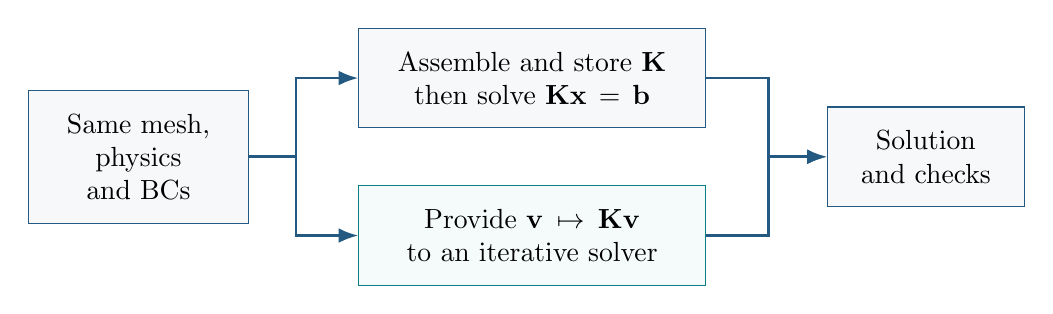
\begin{tikzpicture}[>=Latex]
\node[process,text width=2.2cm] (in) at (0,0) {Same mesh,\\physics and BCs};
\node[process,text width=3.8cm] (asm) at (5,1) {Assemble and store $\mathbf K$\\then solve $\mathbf K\mathbf x=\mathbf b$};
\node[process,text width=3.8cm,draw=teal,fill=teal!4] (mf) at (5,-1) {Provide $\mathbf v\mapsto\mathbf K\mathbf v$\\to an iterative solver};
\node[process,text width=1.9cm] (out) at (10,0) {Solution\\and checks};
\draw[flow] (in.east)--(2,0)|-(asm.west);\draw[flow] (in.east)--(2,0)|-(mf.west);
\draw[flow] (asm.east)--(8,1)|-(out.west);\draw[flow] (mf.east)--(8,-1)|-(out.west);
\end{tikzpicture}\end{center}
\question{What is avoided? What work remains?}
\source{A matrix-free action evaluates the linearised FE operator through local contributions. \phast}
\timing{A 108--114 / 6 minutes}{Explain the action of gather/scatter operators A_e. Assembly, local kernels and boundary handling differ by route. Preconditioning and convergence remain important. Notebook 01 uses assembled SciPy sparse-direct mechanics.}
\end{frame}

\begin{frame}{Tensors still have physical locations}
\begin{tabular}{@{}L{.30\textwidth}L{.26\textwidth}L{.34\textwidth}@{}}
\toprule Field & Typical shape & Meaning\\\midrule
Coordinates & $N\times n_{\rm dim}$ & positions\\[3mm]
Connectivity & $N_e\times n_{\rm loc}$ & local-to-global map\\[3mm]
Displacement, damage & $N\times n_{\rm dim}$; $N$ & nodal fields\\[3mm]
Strain, history & element/quadrature axes & local constitutive state\\\bottomrule
\end{tabular}
\question{Which axes must agree before two tensors can interact?}
\source{Illustrative tensor layouts; inspect array shapes and ordering in the notebook.}
\timing{A 114--120 / 6 minutes}{Retrieval: trace one element from connectivity through quadrature to global accumulation. Identify units and spatial location alongside tensor shapes. Ask why a smooth damage band still needs spatial resolution and numerical convergence. Preview notebook 01.}
\end{frame}

\session{Build, run and differentiate}{Session B / 00--04}{Specify a problem.\\Read its fields and response.\\Check a derivative before recovery.}{Four-minute orientation. Notebook 01 runs PhAST; notebook 02 checks its local degradation law; notebook 03 is a separate original elastic-bar inverse toy. This deliberate scope reduction makes the derivative chain inspectable.}

\begin{frame}{Start from the same computational state}
\tagline{Notebook 01 / setup and version record}
\flowfour{Pinned\\source}{Python /\\PyTorch}{Precision /\\device}{Small\\check}
\vspace{6mm}
\begin{center}\large PhAST 0.16.2\quad\texttt{f6324f899f07}\end{center}
\question{Can you identify the source that was actually imported?}
\source{Load the provided course environment and verify the PhAST source revision. \phast}
\timing{B 04--10 / 6 minutes}{Run the source/version check. The helper gives the vendored manifest precedence and verifies every public source hash, or checks the external public Git revision. Record dtype/device and source version. Setup/download and kernel execution times are different. Saved outputs provide a fallback if setup fails.}
\end{frame}

\begin{frame}{Geometry, mesh and precrack are separate inputs}
\begin{columns}[c]
\begin{column}{.53\textwidth}\fig[.91]{geometry_mesh}\end{column}
\begin{column}{.44\textwidth}
\small Fast route: rectangular T3 mesh from tensors.\par\vspace{4mm}
The precrack is prescribed $d=1$ on centreline nodes.\par\vspace{4mm}
Geometry/import extension: create a Gmsh mesh and inspect named groups.
\end{column}
\end{columns}
\source{Original mesh/BC schematic: symmetric opening and a prescribed damage precrack.}
\timing{B 10--19 / 9 minutes}{Display the actual notebook mesh and node counts. It is a 4 by 2 rectangle, nx=128, ny=64, 8385 nodes and 16384 T3 elements. Damage Dirichlet data prescribe the precrack to x=0.8. The sketch illustrates a coarser T3 mesh with the same symmetric-opening convention as symmetric_tension_bcs. The displayed mesh comes from the structured rectangle generator.}
\end{frame}

\begin{frame}{Boundary sets and prescribed values}
\flowfour{Geometry\\entity}{Mesh\\group}{Selected\\DOFs}{Prescribed\\value}
\vspace{5mm}
\[\texttt{top}\ \longrightarrow\ \{i_1,i_2,\ldots\}\ \longrightarrow\ u_y\ \longrightarrow\ \bar u\]
\question{What happens if the group is empty or the wrong component is fixed?}
\source{Inspect group membership and coordinates before solving. The quick tensor-mesh route identifies boundary node sets; imported meshes require their own group checks.}
\timing{B 19--25 / 6 minutes}{Ask learners to print the count and extent of each boundary set. Check support against rigid-body motion, load direction, corner overlap and prescribed damage. Explain that a physical group carries a name/selection; applying mechanics requires a component and value.}
\end{frame}

\begin{frame}{A reproducible calculation has a complete specification}
\small
\begin{tabular}{@{}L{.30\textwidth}L{.63\textwidth}@{}}
\toprule Input & Tiny public PhAST route\\\midrule
Material / fracture & $E,\nu,G_c,\ell,\eta$; AT2, isotropic degradation\\[3mm]
Mesh / precision & T3; $128\times64$ cells; float64\\[3mm]
Loading & 60 quasi-static increments; symmetric opening\\[3mm]
Numerics & SciPy mechanics; damage/outer tolerances; failure checks\\\bottomrule
\end{tabular}
\question{Which of these choices changes physics? Which changes accuracy?}
\source{Quasistatic AT2 with assembled sparse-direct mechanics. Case values: \texttt{configs/day2\_forward/tiny\_notched\_tension.json}.}
\timing{B 25--33 / 8 minutes}{Read the effective configuration used for the calculation. This quick example uses the isotropic energy form. Point out ell=0.15, eta=1e-7 and stagger tolerance=1e-5. Record solver tolerances and failure flags, then assess discretisation convergence through refinement.}
\end{frame}

\begin{frame}{Distinguish the seeded crack from new damage}
\begin{columns}[c]
\begin{column}{.27\textwidth}
\small AT2 crack cost
\[\begin{aligned}\gamma_\ell(d)&=\frac{d^2}{2\ell}\\&\quad+\frac{\ell}{2}|\nabla d|^2\end{aligned}\]
\[G_c\int_\Omega\gamma_\ell(d)\,\mathrm dx\]
\vspace{3mm}
Seed: prescribed $d=1$\par\vspace{3mm}
History: $d_{n+1}\ge d_n$
\end{column}
\begin{column}{.71\textwidth}\fig[1]{phast_comparison}\end{column}
\end{columns}
\question{What changed after the first increment?}
\source{PhAST quasistatic seeded-crack response over 60 increments; source \texttt{f6324f899f07}.}
\timing{B 33--45 / 12 minutes}{Run the selected notebook or use saved output. These fields were replotted from the frozen NPZ result. First distinguish the locked seed from diffuse regularisation after the first solve, then compare first and final increments. The change beyond the seeded region shows the loading-induced evolution of the diffuse damage field. Use the incremental field in the notebook for a more sensitive view. Compute target 60--120 seconds is a teaching target; receipts describe actual local timings.}
\end{frame}

\begin{frame}{Read response and numerical checks together}
\hspace*{.03\textwidth}\fig[.94]{phast_response}
\question{Does a small residual establish mesh convergence?}
\source{Residuals assess nonlinear solve convergence; assess mesh convergence and physical agreement separately.}
\timing{B 45--55 / 10 minutes}{Read the reaction and recorded outer residual alongside the whole damage field. Inspect bounds, irreversibility and configured failure flags. Discuss why reaction, energy, mesh/load-step sensitivity and a relevant reference answer different questions. The retained record supplies reaction, damage and convergence residuals.}
\end{frame}

\begin{frame}{Change one input, then explain the difference}
\tagline{Five-minute comparison / followed by a ten-minute break}
\flowfour{Predict}{Change\\one input}{Compare\\same scales}{Explain\\one limit}
\vspace{6mm}
\begin{center}\large A material/load change\quad or\quad a numerical refinement\end{center}
\question{Keep the other settings fixed and save both results.}
\source{Changing $\ell$ changes the regularised model; changing $h$ refines its discretisation.}
\timing{B 55--60 / 5 minutes, then break 60--70}{Assign one supported material/load or resolution/tolerance change. Predict direction first. Save both configuration and outputs and compare the same scales. If the second solve is still running, record the state and continue after the break; never imply a result already exists. Take ten minutes.}
\end{frame}

\begin{frame}[fragile]{Tensor code can mirror the finite-element calculation}
\begin{columns}[c]
\begin{column}{.61\textwidth}
\begin{lstlisting}[language=Python]
u_e = u[connectivity]
strain_q = B @ u_e
stress_q = law(strain_q, d_q)
r_e = integrate(B.T @ stress_q)
r = accumulate(r_e, connectivity)
\end{lstlisting}
\end{column}
\begin{column}{.36\textwidth}
Gather\par\vspace{4mm}Local physics\par\vspace{4mm}Weighted quadrature\par\vspace{4mm}Global accumulation
\end{column}
\end{columns}
\question{Where do shape, units and boundary treatment enter?}
\source{Element-level pseudocode; batched implementations combine the same local operations.}
\timing{B 70--78 / 8 minutes}{Trace connectivity, local basis gradients, material state, quadrature weights and global degrees of freedom. Ask the class to name the element and quadrature axes. Explain that tensors expose familiar numerical operations without making all solver operations automatically differentiable.}
\end{frame}

\begin{frame}{A gradient follows a specific computational path}
\tagline{$z_{n+1}=S_n(z_n,p)$; $A_n=\partial S_n/\partial z_n$, $B_n=\partial S_n/\partial p$}
\begin{center}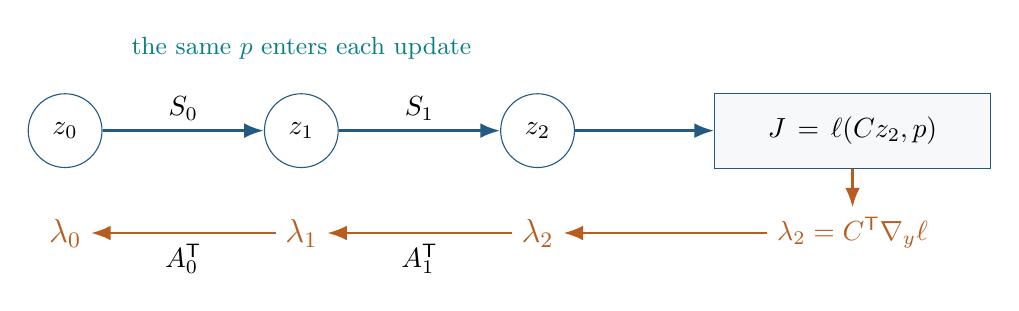
\begin{tikzpicture}[>=Latex]
\foreach \x/\n in {0/0,3/1,6/2}{
 \node[state] (z\n) at (\x,0) {$z_\n$};
 \node[text=reverse,font=\large] (l\n) at (\x,-1.3) {$\lambda_\n$};}
\node[process,text width=2.9cm] (J) at (10,0) {$J=\ell(Cz_2,p)$};
\draw[flow] (z0)--node[above]{$S_0$}(z1);\draw[flow] (z1)--node[above]{$S_1$}(z2);\draw[flow] (z2)--(J);
\node[teal,font=\small] at (3,1.05) {the same $p$ enters each update};
\draw[backflow] (l2)--node[below]{$A_1^{\mathsf T}$}(l1);\draw[backflow] (l1)--node[below]{$A_0^{\mathsf T}$}(l0);
\node[text=reverse] (terminal) at (10,-1.3) {$\lambda_2=C^{\mathsf T}\nabla_y\ell$};
\draw[backflow] (J.south)--(terminal.north);\draw[backflow] (terminal)--(l2);
\end{tikzpicture}\end{center}
\vspace{-2mm}
\[\frac{dJ}{dp}=\underbrace{B_0^{\mathsf T}\lambda_1+B_1^{\mathsf T}\lambda_2}_{\text{add every use of }p}
+\underbrace{\partial_p\ell+(\partial_p z_0)^{\mathsf T}\lambda_0}_{\text{direct and initial-state dependence}}\]
\question{What could break or change this path?}
\source{Custom solves, convergence, boundary treatment, detach, clamps, history maxima and active sets matter. \ad}
\timing{B 78--85 / 7 minutes}{Trace two updates left to right and adjoints right to left. Define fixed C and the scalar final loss. Sum B0 transpose lambda1 and B1 transpose lambda2 because the parameter is shared; retain direct and initial-state terms when present. The optimizer uses the gradient to select an update. The book chapter expands this to three numerical steps with hand/AD/FD checks. p and J here correspond to theta and loss notation elsewhere. Original diagram; visual inspiration: TUM ADL4P Differentiable Physics II, PDF page 5. PyTorch and JAX support differentiable FEM through their automatic-differentiation systems. Check gradients and performance for the implemented computation.}
\end{frame}

\begin{frame}[fragile]{Check a local derivative three ways}
\tagline{Notebook 02 / analytic, automatic, finite difference}
\[g'(d)=-2(1-\eta)(1-d)\qquad
D_\epsilon g(d)=\frac{g(d+\epsilon)-g(d-\epsilon)}{2\epsilon}\]
\begin{lstlisting}[language=Python]
d = torch.tensor(0.25, dtype=torch.float64,
                 requires_grad=True)
(g_ad,) = torch.autograd.grad(material.degradation(d), d)
\end{lstlisting}
\question{Try several $\epsilon$ values. Report precision and error.}
\source{PhAST local degradation law: $\eta=10^{-7}$, $g'(0.25)=-1.49999985$.}
\timing{B 85--97 / 12 minutes}{Execute notebook 02 and compare analytic, AD and central FD. For a quadratic, central FD is exact in real arithmetic; small-step cancellation remains. A nonquadratic smooth extension can demonstrate truncation error. For this exact quadratic, central differences isolate roundoff effects.}
\end{frame}

\begin{frame}{Choose an informative inverse observation}
\tagline{Notebook 03 / elastic-bar parameter recovery}
\[u_{\rm tip}(E)=\frac{FL}{EA}\qquad
\mathcal L(E)=\frac12\sum_j\left[u_{\rm tip}(E;F_j)-u_j^{\rm obs}\right]^2\]
\vspace{4mm}
\flowfour{Guess\\$E>0$}{Solve\\bar}{Compare\\tip response}{Update\\$\log E$}
\question{What is known? Which parameter does the observation constrain?}
\source{Fixed-mesh, one-parameter recovery; optimising $\log E$ preserves positivity.}
\timing{B 97--105 / 8 minutes}{Run the bar exercise, check du_tip/dE against the analytic expression -FL/(AE squared), then recover E. Fix geometry and units. Explain that the scalar toy exposes the parameter-to-loss chain without history maxima, damage constraints or crack-path changes. Full fracture inversion requires its own checks.}
\end{frame}

\begin{frame}{A small loss is only one part of recovery evidence}
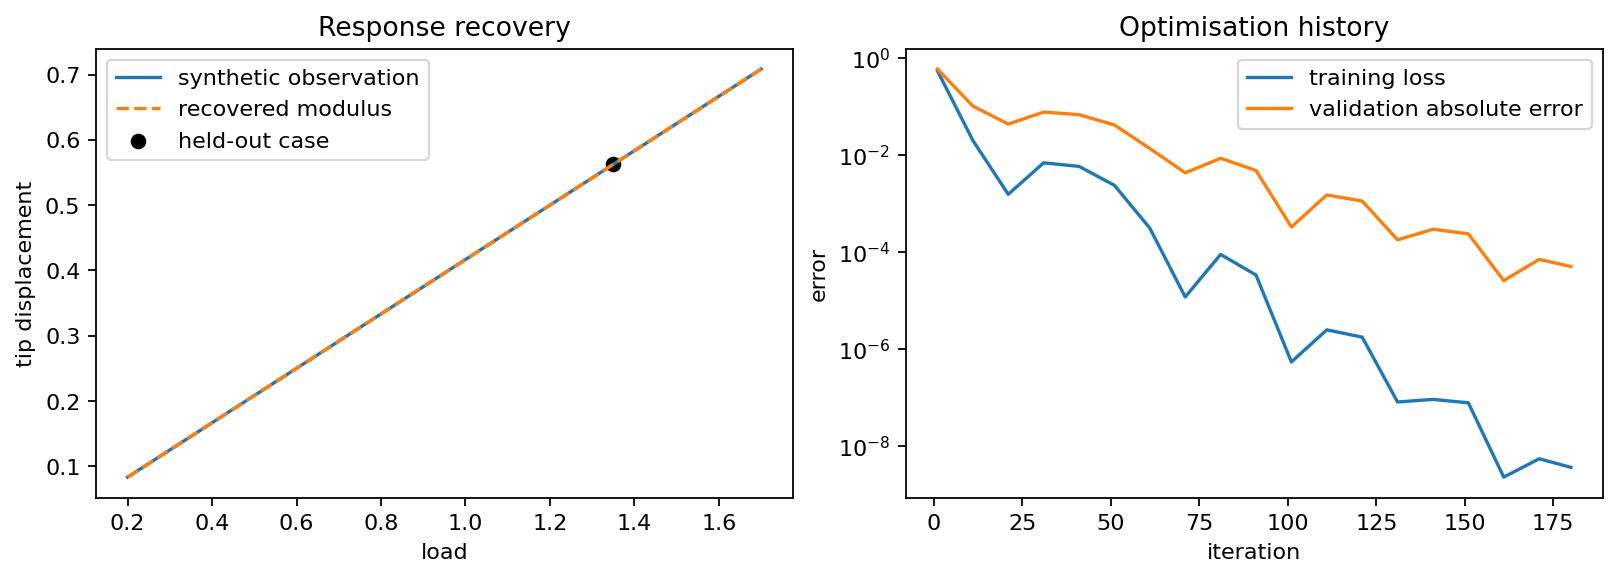
\includegraphics[width=\textwidth]{latex_figures/notebook03_inverse.png}
\question{Check the parameter, the fit and an unused load case.}
\source{Notebook 03: parameter and response recovery for the elastic bar.}
\timing{B 105--110 / 5 minutes}{Inspect actual observations, recovered response, held-out point and optimisation history. Ask for another initial guess where time permits. Inverse uniqueness and recovery depend on observation sensitivity, conditioning and initialisation. The plotted training loss and validation absolute error have different meanings/scales.}
\end{frame}

\begin{frame}{Keep an experiment someone else can reproduce}
\vspace{3mm}
\begin{enumerate}
\item Configuration and source version.\vspace{4mm}
\item Whole field, response and numerical checks.\vspace{4mm}
\item Derivative check and inverse interpretation.
\end{enumerate}
\question{Which conclusion follows from your experiment, and under which assumptions?}
\source{Session B hand-in: one executed notebook and one comparison sheet, including precision, hardware and measured timing scope.}
\timing{B 110--120 / 10 minutes}{Use the final lab block to finish the inverse exercise and hand-in. Record exact inputs, output figures and derivative check. Distinguish the real PhAST forward activity from the elastic-bar inverse toy. Record the execution platform and measured runtime.}
\end{frame}

\session{Train, save and assess a model}{Session C / 00--04}{Fit a compact model.\\Reload the same prediction.\\Assess a proposal and retain correction.}{Four-minute orientation to notebooks 04 and 05. These use synthetic fields from an original Helmholtz-like finite-difference problem. One complete small model is the core learning exercise.}

\begin{frame}{The data card defines what learning means}
\tagline{Notebook 04 / course-owned field equation}
\begin{tabular}{@{}L{.22\textwidth}L{.72\textwidth}@{}}
\toprule Item & Teaching example\\\midrule
Input & Nodewise $[x/L,\ y/H,\ \text{load factor}]$\\[3mm]
Target & A scalar damage-like teaching field\\[3mm]
Split & Whole load cases: train, validation, held-out test\\[3mm]
Provenance & Discrete Helmholtz-like reference equation\\\bottomrule
\end{tabular}
\question{How would correlations between adjacent frames affect a random split?}
\source{Separate whole cases/trajectories to prevent leakage. Feature order, units, location and normalisation are part of the model contract.}
\timing{C 04--10 / 6 minutes}{Read the dataset card before architecture. Explain interpolation and extrapolation and why samples within a case are correlated. The teaching equation supplies its own discrete residual for assessment. Fit normalisation using training data only.}
\end{frame}

\begin{frame}{An MLP maps named features to a named target}
\fig[1]{mlp}
\[\widehat d=\mathcal N_\omega\bigl(\operatorname{normalise}(x/L,y/H,\lambda)\bigr)\]
\question{What physical information is absent from this input?}
\source{A pointwise model uses local input features; graph models additionally encode connectivity.}
\timing{C 10--18 / 8 minutes}{Trace one node through normalisation, hidden layers and output. Identify trainable weights, activation functions and the explicit target. Ask which material, history or boundary information would be needed for a broader fracture problem. Keep the network small enough to inspect in class.}
\end{frame}

\begin{frame}{A fitted model can still miss the local field}
\begin{columns}[c]
\begin{column}{.27\textwidth}
\small Toy reference
\[(\mathbf I+\ell^2\mathbf L_h)d=b\]
\vspace{4mm}
Model
\[\widehat d=\mathcal N_\omega(x/L,y/H,\lambda)\]
\vspace{3mm}
Same held-out load.\par
Same colour scale.
\end{column}
\begin{column}{.71\textwidth}\fig[1]{toy_reference_prediction}\end{column}
\end{columns}
\question{Where is the error concentrated? What does the baseline reveal?}
\source{Notebook 04: Helmholtz-like field prediction at held-out load $\lambda=1$.}
\timing{C 18--30 / 12 minutes}{Run short training, then read actual training/validation logs and the held-out image. The two slide panels show the same held-out reference and reloaded MLP on identical 0--1 scales. Here L_h denotes the positive discrete negative-Laplacian on interior nodes, with boundary rows replaced by Dirichlet conditions; the model map includes the saved feature normalisation. A scalar loss can hide localisation and boundary error. Use the notebook's additional RBF/error panels for diagnosis. Reference generation and training are separate costs.}
\end{frame}

\begin{frame}[fragile]{A checkpoint is more than weights}
\tagline{Notebook 04 / save, new instance, reload, compare}
\begin{columns}[c]
\begin{column}{.57\textwidth}
\begin{lstlisting}[language=Python]
checkpoint = {
    "state_dict": model.state_dict(),
    "architecture": configuration,
    "features": feature_order,
    "normalisation": scaling,
    "source": data_provenance,
}
\end{lstlisting}
\end{column}
\begin{column}{.40\textwidth}
\[\max_i\left|\widehat d_i^{\rm before}-\widehat d_i^{\rm reload}\right|\le\tau\]
\question{Same input. Fresh model. Same prediction.}
\end{column}
\end{columns}
\source{Illustrative checkpoint layout; use the notebook's exact schema. Preserve shape, precision, evaluation mode and supported scope. \ad}
\timing{C 30--45 / 15 minutes}{Execute the actual checkpoint routine. Reconstruct a fresh instance, load weights and metadata, set evaluation mode and compare the same held-out input numerically. Record feature order, normalisation, mesh signature, seed and source. Load checkpoints from a trusted source using the documented format.}
\end{frame}

\begin{frame}{A model swap requires compatible inputs}
\small
\begin{tabular}{@{}L{.25\textwidth}L{.68\textwidth}@{}}
\toprule Representation & Required input construction\\\midrule
MLP / RBF & Named point features; scaling; RBF centres/kernel\\[4mm]
GNN / GNO & Nodes, edges/neighbourhoods and geometry/operator data\\[4mm]
CNN & Grid/channel order and explicit mesh--grid maps\\\bottomrule
\end{tabular}
\question{Try the compatible swap. Deliberately reject an incompatible input.}
\source{The MLP and RBF share one field interface. Mesh transfer requires compatible geometry and discretisation inputs.}
\timing{C 45--60 / 15 minutes, then break 60--70}{Compare the MLP with the compatible RBF and their held-out fields. Check feature ordering, shape, dtype and mesh signature. Explain why a graph or grid model cannot be substituted without constructing its inputs. Deliberately run the notebook incompatibility check. Take the ten-minute break.}
\end{frame}

\begin{frame}{A learned model supplies a proposal}
\tagline{Notebook 05 / a defined teaching adapter}
\flowfour{Current\\state}{Compatible\\features}{Model\\proposal}{Reference\\assessment}
\vspace{6mm}
\begin{center}\large Detached inference and differentiable training use distinct computation graphs\end{center}
\question{What exactly does the adapter promise?}
\source{Notebook 05: model inference followed by residual assessment for the teaching equation.}
\timing{C 70--78 / 8 minutes}{Read the adapter contract: feature order, mesh signature, bounds, output location, precision and scope. The public learned-damage hook uses detached inference. Training through a numerical response requires a connected computational graph. The teaching adapter demonstrates assessment logic on its own equation.}
\end{frame}

\begin{frame}{Admissibility and equilibrium}
\[
d^{\rm proj}=\max\!\left(d^{\rm previous},\ \min(1,\max(0,\widehat d))\right)
\]
\vspace{5mm}
\begin{columns}[t]
\begin{column}{.46\textwidth}
\tagline{Projection can enforce}
$0\le d\le1$\par\vspace{3mm}
$d\ge d^{\rm previous}$
\end{column}
\begin{column}{.48\textwidth}
\tagline{Assessment still asks}
Are the equations satisfied?\par\vspace{3mm}
Are prescribed values consistent?
\end{column}
\end{columns}
\question{Can a bounded field still be mechanically wrong?}
\source{Assess admissibility, residual convergence and energy consistency with criteria appropriate to the model.}
\timing{C 78--85 / 7 minutes}{Explain the nested min/max operation and consistent boundary treatment. The algebraic projection enforces simple bounds and irreversibility. A separate residual assessment checks equilibrium. A fracture active-set problem needs a suitable projected/KKT check. The teaching equation has its own defined residual.}
\end{frame}

\begin{frame}{Acceptance needs an explicit correction route}
\begin{center}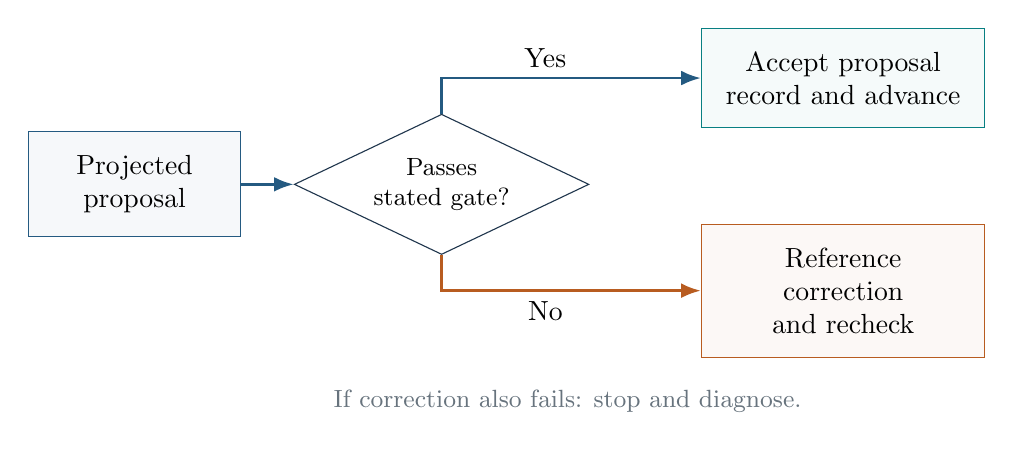
\begin{tikzpicture}[>=Latex]
\node[process] (p) at (0,0) {Projected\\proposal};
\node[decision] (q) at (3.9,0) {Passes\\stated gate?};
\node[process,draw=teal,fill=teal!4,text width=3cm] (a) at (9,1.35) {Accept proposal\\record and advance};
\node[process,draw=reverse,fill=reverse!4,text width=3cm] (r) at (9,-1.35) {Reference\\correction\\and recheck};
\draw[flow] (p)--(q);
\draw[flow] (q.north)|-node[above,pos=.7]{Yes}(a.west);
\draw[backflow] (q.south)|-node[below,pos=.7]{No}(r.west);
\node[font=\small,muted] at (5.5,-2.75) {If correction also fails: stop and diagnose.};
\end{tikzpicture}\end{center}
\question{Inspect one useful proposal and one rejected proposal.}
\source{Record the proposal, projection, residual, decision, correction and total computational cost.}
\timing{C 85--90 / 5 minutes}{Run notebook 05 and read its useful/rejected proposal comparison and correction record. The deliberately corrupted input should trigger reference fallback. Include proposal, audit and correction in any timing comparison; compare complete computational routes at matched accuracy.}
\end{frame}

\begin{frame}{DAgger learns from states the model visits}
\tagline{Conceptual extension: the current notebook saves one replay record}
\begin{center}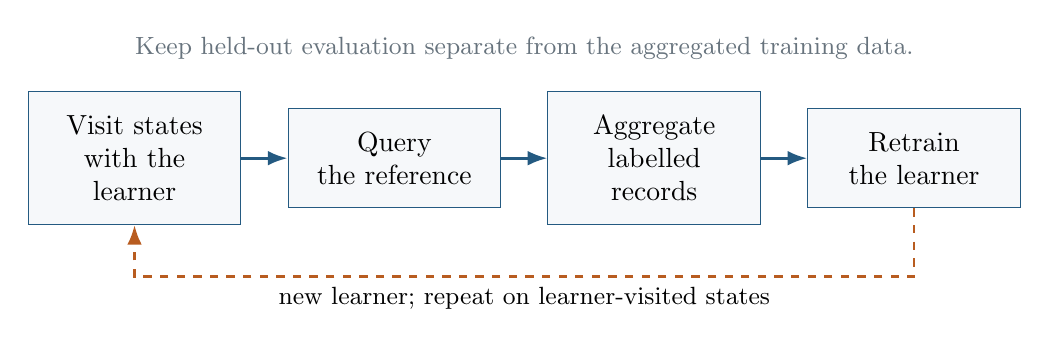
\begin{tikzpicture}[>=Latex]
\node[process] (v) at (0,0) {Visit states\\with the learner};
\node[process] (q) at (3.3,0) {Query\\the reference};
\node[process] (a) at (6.6,0) {Aggregate\\labelled records};
\node[process] (t) at (9.9,0) {Retrain\\the learner};
\draw[flow] (v)--(q);\draw[flow] (q)--(a);\draw[flow] (a)--(t);
\draw[backflow,dashed] (t.south)--(9.9,-1.5)--node[below,font=\small]{new learner; repeat on learner-visited states}(0,-1.5)--(v.south);
\node[muted,font=\small] at (4.95,1.4) {Keep held-out evaluation separate from the aggregated training data.};
\end{tikzpicture}\end{center}
\question{How do visited states differ from teacher-provided states?}
\source{\daggerref\quad Inspect the saved replay record and design one data-aggregation round.}
\timing{C 90--105 / 15 minutes}{Explain Dataset Aggregation: roll out the learner, obtain expert/reference labels on learner-induced states, append training data, retrain and evaluate on unchanged held-out cases. Inspect the saved correction/replay record. The notebook supplies a correction and replay record for discussing data aggregation. Optional activity: design one controlled offline round and its cost/evaluation gates.}
\end{frame}

\begin{frame}{Architectures encode different assumptions}
\begin{tabular}{@{}L{.27\textwidth}L{.66\textwidth}@{}}
Point map & Compact features; explicit coordinate assumptions\\[5mm]
Grid or graph & Structured stencil or irregular neighbourhood\\[5mm]
Operator map & Function inputs/outputs; training and discretisation scope\\
\end{tabular}
\question{Which new load, material, mesh or topology has actually been tested?}
\source{Choose a representation for the input structure, discretisation and intended evaluation setting.}
\timing{C 105--110 / 5 minutes}{Compare input construction and inductive assumptions. Moving from the small toy to fracture needs material/history/boundary representation and an appropriate data split. Assess transfer using held-out topologies, loading cases and crack paths.}
\end{frame}

\begin{frame}{Read a research example through the same evidence}
\vspace{4mm}
\begin{enumerate}
\item Whole field and physical load/time history.\vspace{4mm}
\item Matched response, numerical checks and held-out scope.\vspace{4mm}
\item Source/configuration and complete computational cost.
\end{enumerate}
\question{What has this example demonstrated, specifically?}
\source{Research discussion: compare the physical problem, numerical method, accuracy and computational cost.}
\timing{C 110--115 / 5 minutes}{Use a course-lead-supplied permitted paper example if available. Use the approved public examples in the companion material. Compare like accuracy, hardware and precision; include data/reference generation, training, prediction, audit and correction when relevant. Use matched timings to evaluate computational cost.}
\end{frame}

\begin{frame}{A useful contribution starts with reproducibility}
\flowfour{Practise\\an extension}{Reproduce\\a small case}{Explain\\the result}{Contribute\\docs or code}
\vspace{6mm}
\begin{center}\large\href{https://github.com/CEMS-Lab/PhAST}{github.com/CEMS-Lab/PhAST}\end{center}
\question{What is the smallest example another person could run?}
\source{Read current contribution and issue guidance before submitting. Keep private data, credentials and unpublished results out of public reports.}
\timing{C 115--118 / 3 minutes}{Suggest a documentation correction, exercise extension or minimal reproducible issue. Include environment/source, configuration, expected/actual behaviour and relevant output. Students can submit a reproducible issue or contribution through the repository.}
\end{frame}

\begin{frame}{Keep the chain from assumptions to evidence visible}
\begin{tabular}{@{}L{.07\textwidth}L{.85\textwidth}@{}}
\color{teal}A & Representation $\to$ energy $\to$ discretisation\\[5mm]
\color{teal}B & Configuration $\to$ result $\to$ derivative\\[5mm]
\color{teal}C & Data $\to$ prediction $\to$ assessment\\
\end{tabular}
\vspace{4mm}
\question{Name one physical assumption, one check and one limitation.}
\source{References and further reading: \texttt{slides/README.md} and the companion book. Original course graphics.}
\timing{C 118--120 / 2 minutes}{Close with retrieval of the main ideas. The PDF is the teaching copy and the TeX/Matplotlib files are the editable source. Point to the companion book and all five notebooks. The teaching sequence draws inspiration from CWI's physical examples, small training loops and model-induced-state assessment. The course visuals are original.}
\end{frame}

\end{document}
